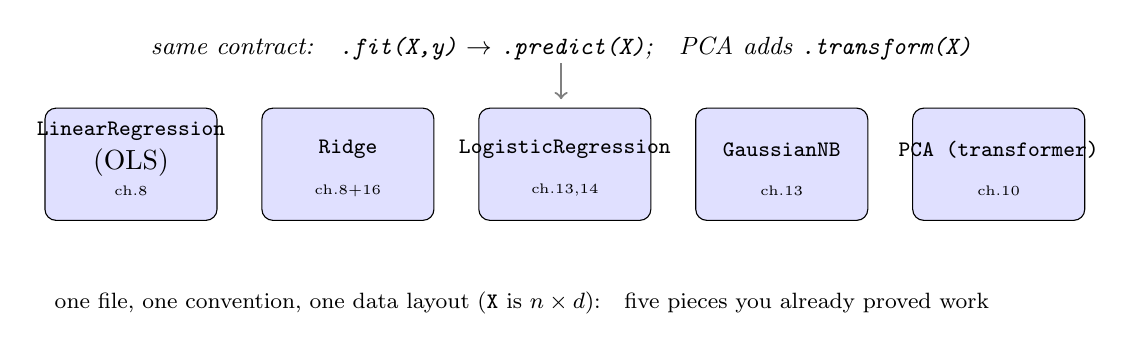
\begin{tikzpicture}[scale=0.95, every node/.style={align=center}]
\foreach \x/\name/\ch in {0/{LinearRegression}\\{(OLS)}/{ch.8},
  2.9/{Ridge}/{ch.8+16},
  5.8/{LogisticRegression}/{ch.13,14},
  8.7/{GaussianNB}/{ch.13},
  11.6/{PCA (transformer)}/{ch.10}}{
  \draw[fill=blue!12, rounded corners] (\x,0) rectangle
    ({\x+2.3},1.5);
  \node at ({\x+1.15},0.95) {\footnotesize\ttfamily\name};
  \node[font=\tiny] at ({\x+1.15},0.4) {\ch};
}
\node[font=\small\itshape] at (6.9,2.3) {same contract:\quad
  \texttt{.fit(X,y)} $\to$ \texttt{.predict(X)};\quad PCA adds
  \texttt{.transform(X)}};
\draw[->, thick, gray] (6.9,2.1) -- (6.9,1.62);
\node[anchor=west, align=left] at (0,-1.1) {\footnotesize one file,
  one convention, one data layout (\texttt{X} is $n\times d$):\quad
  five pieces you already proved work};
\end{tikzpicture}
